\chapter{Shrinkage Methods} \label{ch:shrinkageMethods}
Shrinkage Methods penalizes the coefficient by shrinking the coefficients towards zero. Using this techniques that can reduce the variance of the model. 

\section{Theory}
\subsection{Vector norm}
A norm is a function that gives a positive length to each vector in a vector space.

\noindent Using the P-norm $\lVert X \rVert_p = (\sum_{i=1}^{n}|x_i|^p)^{1/p}$.\footnote{https://www.wikiwand.com/en/Norm\_(mathematics)} If we set $ p = 1 $ we get the first norm also called the Manhattan norm. It got it's name because it works similarly to how a taxi would drive in New York City always in a grid-like route 1 block to the east then 2 block to the north. The second norm is called Euclidean distance and that is the distance in a straight line just as a bird would fly. Both norms can be seen visually on Figure \ref{fig:normfirstsecond}\footnote{\cite{James2013} p. 222}.

\begin{figure}[H]
	\centering
	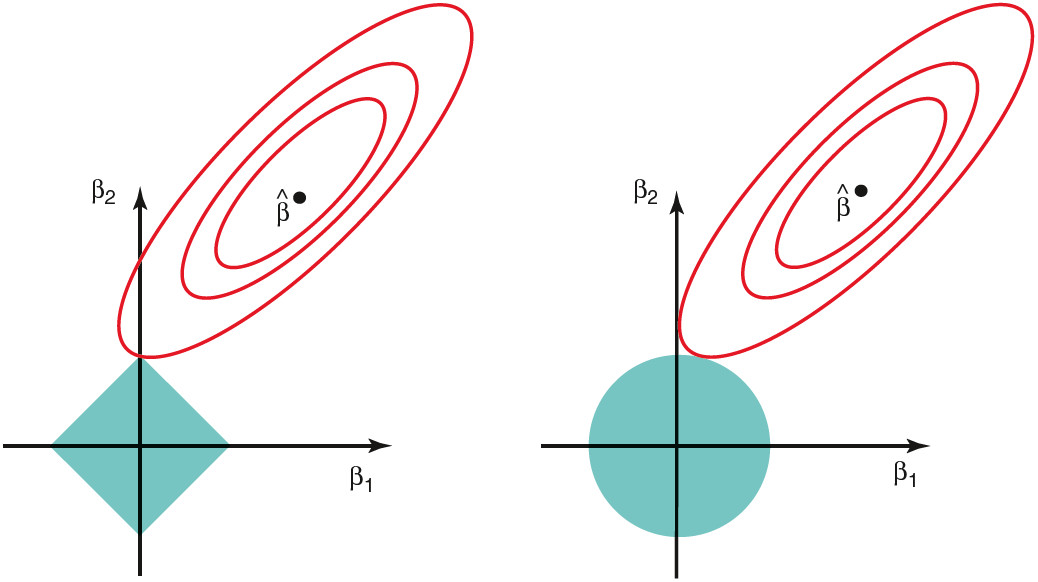
\includegraphics[width=0.5\textwidth]{shrinkageMethods/fig/normsL1_L2.jpg}
	\caption{The red eclipse shows the concurs of ridge (left) and lasso (right) regression. The blue areas are constraint regions for the first and second norm. Notice that lasso intersects the constraint region at an axis, whereas ridge does not.}
	\label{fig:normfirstsecond}
\end{figure}

\subsection{Ridge regression}
The formula for Ridge regression can be seen in Formula \ref{fo:RidgeRegression}. The blue part represent the residual sum of square (RSS) term and the red part represent the regularize or penalty term. The penalty term is small when $\beta_1, \ldots ,\beta_p$ are close to zero and it has the effect of shrinking or penalizing the estimates of the coefficients $\beta_j$ towards zero. $\lambda$ also called a tuning parameter decides how much impact the two terms get. If $\lambda = 0$ then we will only get least squares estimates, but as $ \lambda \to \infty$ the penalty terms influence will increase and therefore the coefficients will approach zero. This means that the results will be different depending on the chosen $\lambda$ so for getting a good result picking the right $\lambda$ is important.

\noindent The penalty term only apply to the slope, not the intercept. $\lambda$ in in \ref{fo:RidgeRegression} control the degree of penalty.
\begin{align}\label{fo:RidgeRegression}
\color{blue} \sum_{i=1}^{n} ( y_i - \beta_0 - \sum_{j=1}^{p} \beta_j x_i,j )^2 \color{black} + \color{red} \lambda \sum_{j=1}^{p} \beta^2_j 
\end{align}
The reason to Ridge regression over least squares is found in the bias-variance
trade-off. This is because as our $\lambda$ gets bigger the complexity of the ridge regression fit decreases leading to less variance but more bias.

\subsection{The lasso regression}
The formula for least absolute shrinkage and selection operator, also called Lasso, can be seen in Equation \ref{fo:TheLasso}. The blue part of the equation is the RSS and the red part is the penalty-term. The Lasso regression has a advantage over Ridge regression because of the way the penalty term works. In Ridge it will include all $p_i$ predictors because the $\lambda \sum_{j=1}^{p} \beta^2_j$ only shrink all of the coefficients towards zero. In lasso we use the $\ell_1$ norm, the coefficient vector $\beta$ is given by $ \lVert \beta_1 \rVert = \sum | \beta_j |$ which results in some of the coefficient estimates to be exactly zero, when the tuning parameter $\lambda$ is large enough.
\begin{align}\label{fo:TheLasso}
\color{blue} \sum_{i=1}^{n} ( y_i - \beta_0 - \sum_{j=1}^{p} \beta_j x_i,j )^2 \color{black} +  \color{red} \lambda \sum_{j=1}^{p} |\beta_j|
\end{align}
Because the lasso regression removes some of the coefficients, lasso models are generally easier to understand than Ridge regression models, because they are more sparse with a reduced complexity. Lasso models involve only a subset of the variables. Like before selecting a good $\lambda$ is important here.

\subsection{Comparing ridge and lasso regression}

From equations \ref{fo:RidgeRegression} and \ref{fo:TheLasso} we see that a Lasso regression model could potentially end up with less variables than Ridge regression, since the coefficients can be forced to equal zero, because of the $\ell_1$ penalty. This is called sparsity. You would typically use Ridge regression to prevent over-fitting, since it keeps all features, but can prove less useful with a large number of features (\textit{p} > \textit{n}). On the other hand, Lasso is useful when you have many features and provides you with a more sparse model that could give a computational advantage. Ridge regression generally performs better in terms of bias, variance and MSE when the predictors are related to the response. %However if the response is just a subset of the original predictors, we tend to get better results with Lasso regression.
%TODO Confusing conclussion

\section{Results}
\subsubsection*{LAB 6.6.1}
Lab 6.6.1\footnote{Appendix 13 - 6.6.1 Ridge Regression} uses Ridge Regression on the hitters dataset. Using scikit-lean and their implementation. Some players were missing salary, therefor these were dropped out. The data also contained some string values and using pandas they were converted  into dummy variables.  
\begin{figure}[H]
	\centering
	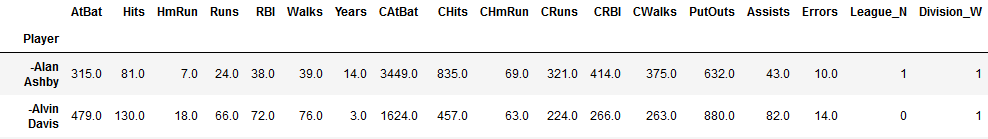
\includegraphics[width=0.8\textwidth]{shrinkageMethods/fig/data.png}
	\caption{The data after removing missing values and making strings into dummy variables }
	\label{fig:lab661_data}
\end{figure}
The data were spited into a training and test set. Then it ran Ridge Regression with a alpha of 4 and displayed mean squared error.


\noindent\textit{MSE= 134512.83820473132}

Afterwards displayed some coefficients.

\noindent\textit{AtBat  -2.185390}

\noindent\textit{Hits    7.392346}

\noindent\textit{HmRun  -2.666724}

If the same code would be run again but with a alpha that is very large $10^10$ then are coefficients get even smaller.

\noindent\textit{AtBat  5.135079e-04}

\noindent\textit{Hits    1.771301e-04}

\noindent\textit{HmRun  2.568334e-05}

And  MSE also gets even higher.

\noindent\textit{MSE= 211698.60251243794}

As discussed in the theory and see just before picking the right alpha part of this is important.The cross validation is used to find the best alpha using scikit learn's RidgeCV. That is Ridge regression with built-in cross-validation. Which has displayed 

\noindent\textit{2.3570694139967037}

After finding the best alpha using the cross validation the code was ran again with the new alpha.   

\noindent\textit{134355.75204499933}

Using a plot it is also seen that trends coefficients move toward zero.
\begin{figure}[H]
	\centering
	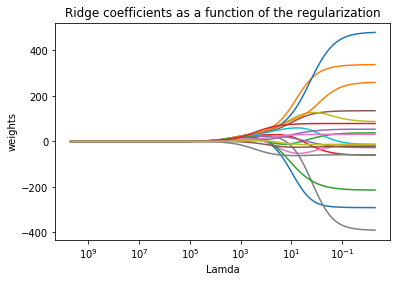
\includegraphics[width=0.45\linewidth]{shrinkageMethods/fig/plot}
	\caption{Ridge regression on the hitters dataset}
	\label{fig:plot}
\end{figure}
Lab 6.6.2\footnote{Appendix 14 - 6.6.2 The Lasso} uses The Lasso and the same steps to prepare the dataset as before. In Lasso there is a need to find best alpha and the fastest way is to use LassoCV that has cross validation built ind.

\noindent\textit{1072.2672220103254}

Also some of the coefficients are displayed, some of them are zero just as described in the theory section.

\noindent\textit{AtBat          0.729684}

\noindent\textit{Hits           0.000000}

\noindent\textit{HmRun         -0.000000}

\noindent\textit{Runs           0.000000}